% !TEX root = ../00_thesis.tex


%-------------------------------------------------------------------------------
\subsection{Simulated Worst-Case Performance}
\label{subsec:simulation}

In \cref{subsec:perf_model}, we derived the optimal performance achievable according to our \DRP's model.
However, this model is based on a worst-case analysis of message latency throughout the system.
Because such an analysis is inherently pessimistic, it is important to estimate how pessimist the analysis is. In other words, how tight are the latency bounds given by the model?
In this section, we investigate this question using a discrete event simulation.

\fakepar{Procedure}
We simulate the run-time behavior of \DRP using the values and parameters from our implementations~(\cref{table:simulation_parameters}).
The simulation framework tracks the latency of each individual message through the entire system, \ie all \APs, \CPs, \bolt and the wireless communication network.
Concretely, the simulation is implemented using Matlab scripts (openly available -- \cref{append:drp_artifacts}).

\blink computes the round schedules assuming that the first message of each flow is available for communication at $t = 0\s$. The actual epoch at which the  \APs write the first packet of each flow is randomized between $0\s$ and the flow's minimal message interval $T$; subsequent packets are sent with period $T$.
The random seed is fixed for reproduciblility.

\fakepar{Scenario}
Node 1 acts as the sink and communicates with all other nodes in the network. As described in \cref{sec:designDetailed}, \DRP is initialized with a set of control flows $\mathcal{F}_{control}$, which is necessary in order to register subsequent flows
\[
\mathcal{F}_{control} =
	\left\lbrace
	\begin{tabular}{@{\,}l@{\,}}
	(1\,, n\,, \periodany = 10\s\,, \jitterany = 0\s\,, \deadlineany = 30\s )\\
	(n\,, 1\,, \periodany = 10\s\,, \jitterany = 0\s\,, \deadlineany = 30\s )\\
	\end{tabular}
	\right\rbrace
\]
for $n \in ($2$ .. $20$)$. In practice, such flows can also be used to send low-priority data (\eg status data) regularly to the sink.

An event from the environment (\eg a rock crack~\cite{meyer2019IPSN}) is co-detected by nodes 2 to 5, which consequently emit a request for a new flow to the sink node. In order to transfer the event data as fast as possible, the message interval is chosen as small as possible
(\ie equal to $T_f^s$, the flushing interval of $\cp$ -- Refer to \eqref{eq:design_flush_period_source}, \eqref{eq:design_round_period} and \eqref{eq:ndeadline_constraint_period}),
\[
\mathcal{F}_{new} =
	\left\lbrace
	\begin{tabular}{@{}l@{}}
	(n\,, 1\,, \periodany = 1.074\s\,, \jitterany = 0\s\,, \deadlineany = 10\s )\\
	\end{tabular}
	\right\rbrace
\]
for $n \in ($2$ .. $5$)$. We record the end-to-end latency of all packets during two minutes, during which about 900 messages are transmitted through the system.

\fakepar{Results}
\cref{fig:latency} shows the distribution of end-to-end latency of messages, shown as percentage of the analytical worst-case latency (given by \cref{thm:delta}).
We see that a few messages indeed experience a latency up to 97\,\% of the analytic worst-case bound.
The simulation also indicates that, in many cases, the worst-case buffer sizes of $\cp$ and \bolt are reached.
Overall, these results support our analysis of \DRP. They show that our worst-case bounds are tight; therefore, we can conclude that the performance derived using \DRP's model~(\cref{subsec:perf_model}) is representative of the performance that can be truly guaranteed by the system.


\begin{figure}
	\centering
	\href{\drpfig{Figure-11}}{%
	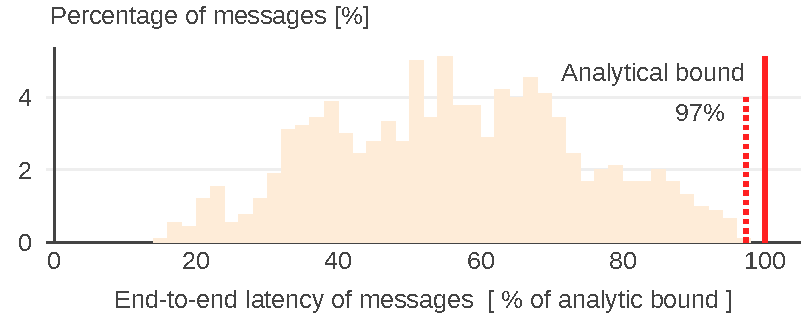
\includegraphics[scale=1]{lat_simu}}
	\caption{Distribution of end-to-end latency of messages, shown as percentage of the analytical worst-case latency.
		\capt{Some messages experience a latency very close to their worst-case bound (97\,\%), which demonstrates the tightness of the analysis.}
	 }
	\label{fig:latency}
\end{figure}

%-------------------------------------------------------------------------------
\subsection{Real-World Performance}
\label{subsec:flocklab}

\begin{table}
	\caption{Flow sets used in the end-to-end latency evaluation of \DRP.
	\capt{The \blink utilization is computed assuming a strictly periodic release of messages.}}
	{\smaller\input{\PathTab/flow_set.csv}}
	\label{tab:flow_set}
\end{table}

% Some intro about why we do real tests
We now consider the performance of our implementation of \DRP on embedded hardware: We use the first-generation DPP, which features a TI MSP432P401R as \AP and a TI CC430F5147 as \CP~(\cref{append:dpp}).
The software is based on the publicly available implementation of LWB~\cite{Code_LWB}; it is written in C and uses Contiki 2.7~\cite{contiki} as operating system.
The implementation of \blink on the \AP is built upon~\cite{acevedo2016Realtime}.
%
We discuss our implementation performance in terms of memory usage, computation workload, and message latency.

\fakepar{Memory usage}
\DRP requires both \AP and \CP to store some state information related to the currently running flows, as well message queues and buffers. The available RAM on both processors is shown in \cref{table:memory}.

The 64\kB of the \AP are largely sufficient; it would supports hundreds of flows. The \CP is more limited: With a payload size of 32\bytes, \CP is capped to a maximum for 40 flows~(\cref{table:memory}). For a regular node, this will likely be sufficient for most applications; however, on the host node, this seriously limits the scalability of the system.

One possible solution is to use the embedded external memory (128\kB); this would solve the memory limitation issue, but it may also introduce additional delays, which are currently not accounted for. Or we could use another processor as \CP with more than 4\kB of RAM.

\begin{table}
	\centering
	\caption{Memory available and required for our implementation of \DRP.
	\capt{%
		The difference between ``total'' and ``available''  memory corresponds to the memory taken by the firmware only. $L$ is the message payload.}
	}
	\label{table:memory}
	{\smaller\input{\PathTab/memory.csv}}
\end{table}


\fakepar{Computation}
The most extensive computations in \DRP are the computations of the \blink schedules and admission tests. The evaluation of these computations on embedded hardware is discussed in depth in~\cite{zimmerling2017Blink}.

In addition to \blink computations, the \APs must perform \DRP admission tests. These are simple operations~(\cref{thm:CP} and \ref{thm:AP}) which can be implemented efficiently. In our experiments, an admission test takes typically around 30\ms to complete (maximum observed execution time: 130\ms).

\DRP admission tests are performed only once per flow (when a new flow is requested). Thus, we can conclude that the computational workload induced by \DRP (in addition to \blink) is negligible.

\afterpage{
\begin{figure}
	\centering
		\begin{subfigure}{\linewidth}
				\captionsetup{labelformat=empty}
				\href{\drpfig{Figure-12}}{%
	      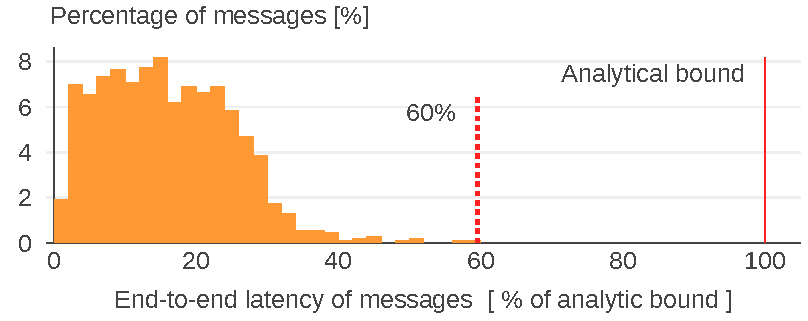
\includegraphics[scale=1]{lat_real_low}}
				\caption{}
			\end{subfigure}\\[10pt]
			\begin{subfigure}{\linewidth}
					\captionsetup{labelformat=empty}
					\href{\drpfig{Figure-12}}{%
		      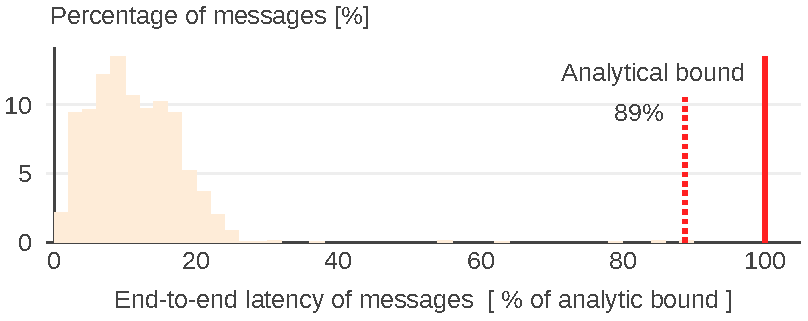
\includegraphics[scale=1]{lat_real_medium}}
					\caption{}
				\end{subfigure}\\[10pt]
				\begin{subfigure}{\linewidth}
						\captionsetup{labelformat=empty}
						\href{\drpfig{Figure-12}}{%
			      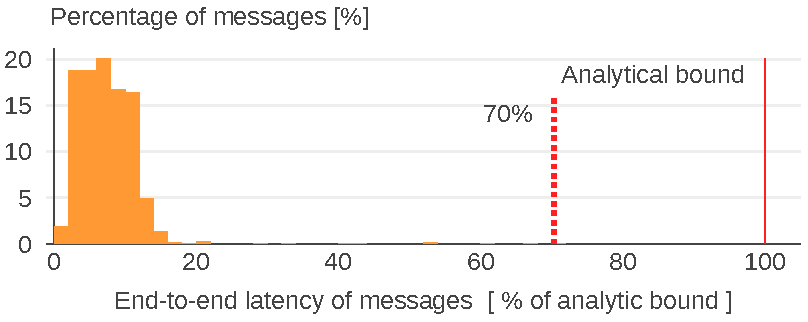
\includegraphics[scale=1]{lat_real_high}}
						\caption{}
					\end{subfigure}
  \caption{%
	Distribution of end-to-end latency of messages, shown as percentage of the analytical worst-case latency for a \DRP run using different flow sets~(\cref{tab:flow_set}).
	\capt{%
	Top -- Low utilization.
	Middle -- Medium utilization.
	Bottom -- High utilization.}
  }
  \label{fig:lat_real_all}
\end{figure}
}


\fakepar{End-to-end latency}
We investigate the experienced end-to-end latency of messages. We use a network of 10 source nodes and one host, and run experiments on the FlockLab testbed~\cite{lim2013FlockLab}. In addition to the control flows, each source node request a data flow toward the host with a pseudo-random period and end-to-end deadline.
Once the flow is admitted, the source \APs release new packets periodically.
The different flow sets used are listed in \cref{tab:flow_set}. \DRP is configured with a deadline ratio $r=0.5$, a round length $\rlength = 1\s$, and a maximum of $\nslotsmax = 5$ slots per round.


\begin{table}
	\centering
	\caption{Experienced latency of messages, expressed as percentage of the flow's end-to-end deadline.
	\capt{The tightness correspond to the ratio of the experienced latency with the analytical upper-bound given by~\cref{thm:delta}.}}
	{\smaller\input{\PathTab/latency.csv}}
	\label{tab:latency}
\end{table}


The results are summarized in \cref{tab:latency} and \cref{fig:lat_real_all}, reporting data from one run for each flow set.
The first observation is that all messages that are successfully transmitted over the wireless network do meet their end-to-end deadline.
However, compared to the simulation experiment~(\cref{subsec:simulation}), we do not encounter so much analytical corner cases: the observed latency is often much smaller than the analytical upper-bound~(\cref{fig:lat_real_all}).
On the other hand, this means that the actual runtime performance is better that what is guaranteed: even with large end-to-end deadlines (around 60\s), the experience message latency is most of the time between 5\s to 15\s.

Such ``short'' average latency can be explained by the nature of the flow set. The \emph{network} deadline, enforced by \blink, must be smaller than the flow period~\cref{sec:designDetailed}. Since the period are small compared to the \emph{end-to-end deadlines}, these end-to-end deadlines do not constraint the \DRP contracts: the experience latency correlates with the flow period.

It is interesting to observe that the average end-to-end latency is smaller for the high utilization flow set than for the low and middle ones. Again, this is due to the flow set. To meet the network deadline, \blink schedule at least one round per period. Thus, a flow set with shorter period results in more frequent rounds. Once a round is scheduled, it is filled with any message ready for transmission. Thus, flows are opportunistically served earlier than necessary to meet their end-to-end deadline. Conclusion: having a flow with a small period reduces the average latency experienced by all flows in the system. This is an interesting (and unforeseen) consequence of \DRP mechanism.

\fakepar{Conclusions}
The performance evaluation presented in this section validates the design of \DRP and our implementation: we showcased that we can run a wireless \CPS that meet end-to-end deadlines between distributed applications~(\cref{subsec:simulation} and \ref{subsec:flocklab}).
In addition, we derived the theoretical optimal performance achievable based on \DRP's model~(\cref{subsec:perf_model}).

A more thorough investigation of the actual system performance across different scenarios and environments remains to be performed.
For such a performance evaluation, using \triscale~(\cref{ch:triscale}) would be natural.

Chronologically, \triscale is the last piece of work of this dissertation. In hindsight, our evaluation of \DRP appears a bit naive and simple. Still, we argue that it successfully demonstrates the soundness of \DRP's design.% and supports our claims.
